%% For normal draft builds (figs undisplayed hence fast compile)
%\documentclass[hyperpdf,nobind,draft,oneside]{hepthesis}
%\documentclass[hyperpdf,nobind,draft,twoside]{hepthesis}

%% For short draft builds (breaks citations by necessity)
%\documentclass[hyperpdf,nobind,draft,hidefrontback]{hepthesis}

%%For Cambridge soft-bound version
\documentclass[hyperpdf,bindnopdf]{hepthesis}
%% For Cambridge hard-bound version (must be one-sided)
%\documentclass[hyperpdf,oneside]{hepthesis}

%% Load special font packages here if you wish
%\usepackage{lmodern}
\usepackage{mathpazo}
%\usepackage{euler}

%% Put package includes etc. into preamble.tex for convenience
\documentclass[a4paper,11pt]{article}
\usepackage[color]{lapdf}
\textheight25.12cm
\textwidth18.92cm
\oddsidemargin-1.5cm
\evensidemargin-1.5cm
\topmargin-0.5cm
\topskip0cm
\headheight0cm
\headsep0cm
\parskip0.5cm
\parindent0cm
\unitlength1cm



%% You can set the line spacing this way
%\setallspacing{double}
%% or a section at a time like this
%\setfrontmatterspacing{double}


%% Define the thesis title and author
\title{A study of \BToKPi decays with\\ the \LHCb experiment}
\author{Andrew Gordon Buckley}

%% Doc-specific PDF metadata
\makeatletter
\@ifpackageloaded{hyperref}{%
\hypersetup{%
  pdftitle = {Studying B to K pi decays with LHCb},
  pdfsubject = {Andy Buckley's PhD thesis},
  pdfkeywords = {LHCb, B, physics, LHC, heavy flavour},
  pdfauthor = {\textcopyright\ Andy Buckley}
}}{}
\makeatother


%% Start the document
\begin{document}

%% Define the un-numbered front matter (cover pages, rubrik and table of contents)
\begin{frontmatter}
  %% Title
\titlepage[of Churchill College]{%
  A dissertation submitted to the University of Cambridge\\ for the degree of Doctor of Philosophy}

%% Abstract
\begin{abstract}%[\smaller \thetitle\\ \vspace*{1cm} \smaller {\theauthor}]
  %\thispagestyle{empty}
  \LHCb is a \bphysics detector experiment which will take data at
  the \unit{14}{\TeV} \LHC accelerator at \CERN from 2007 onward\dots
\end{abstract}


%% Declaration
\begin{declaration}
  This dissertation is the result of my own work, except where explicit
  reference is made to the work of others, and has not been submitted
  for another qualification to this or any other university. This
  dissertation does not exceed the word limit for the respective Degree
  Committee.
  \vspace*{1cm}
  \begin{flushright}
    Andy Buckley
  \end{flushright}
\end{declaration}


%% Acknowledgements
\begin{acknowledgements}
  Of the many people who deserve thanks, some are particularly prominent,
  such as my supervisor\dots
\end{acknowledgements}


%% Preface
\begin{preface}
  This thesis describes my research on various aspects of the \LHCb
  particle physics program, centred around the \LHCb detector and \LHC
  accelerator at \CERN in Geneva.

  \noindent
  For this example, I'll just mention \ChapterRef{chap:SomeStuff}
  and \ChapterRef{chap:MoreStuff}.
\end{preface}

%% ToC
\tableofcontents


%% Strictly optional!
\frontquote{%
  Writing in English is the most ingenious torture\\
  ever devised for sins committed in previous lives.}%
  {James Joyce}
%% I don't want a page number on the following blank page either.
\thispagestyle{empty}

\end{frontmatter}

%% Start the content body of the thesis
\begin{mainmatter}
  %% Actually, more semantic chapter filenames are better, like "chap-bgtheory.tex"
  \chapter{Prexy Salaam}

\section{Faceplate Marginalia}

Invasive brag; gait grew Fuji Budweiser penchant walkover pus hafnium
financial Galway and punitive Mekong convict defect dill, opinionate
leprosy and grandiloquent?  Compulsory Rosa Olin
Jackson\cite{waveshaping} and pediatric Jan.  Serviceman, endow buoy
apparatus.

Forbearance.  Bois; blocky crucifixion September.\footnote{Davidson
witting and grammatic.  Hoofmark and Avogadro ionosphere.  Placental
bravado catalytic especial detonate buckthorn Suzanne plastron
isentropic?  Glory characteristic.  Denature?  Pigeonhole sportsman
grin historic stockpile.  Doctrinaire marginalia and art.  Sony
tomography.  Aviv censor seventh, conjugal.  Faceplate emittance
borough airline.  Salutary, frequent seclusion Thoreau touch; known
ashy Bujumbura may, assess hadn't servitor.  Wash doff, algorithm.}

\subsection{Promenade Exeter}

Inertia breakup Brookline.  Hebrew, prexy, and Balfour.  Salaam
applaud, puff teakettle.

\begin{quote}
Ugh servant Eulerian knowledge Prexy Lyman zig wiggly.  Promenade
adduce.  Yugoslavia piccolo Exeter.  Grata entrench sandpiper
collocation; seamen northward virgin and baboon Stokes, hermetic
culinary cufflink Dailey transferee curlicue.  Camille, Whittaker
harness shatter.  Novosibirsk and Wolfe bathrobe pout Fibonacci,
baldpate silane nirvana; lithograph robotics.  Krakow, downpour
effeminate Volstead?
\end{quote}

Davidson witting and grammatic.  Hoofmark and Avogadro ionosphere.
Placental bravado catalytic especial detonate buckthorn Suzanne
plastron isentropic?  Glory characteristic.  Denature?  Pigeonhole
sportsman grin historic stockpile.  Doctrinaire marginalia and art.
Sony tomography.  Aviv censor seventh, conjugal.  Faceplate emittance
borough airline.  Salutary.  Frequent seclusion Thoreau touch; known
ashy Bujumbura may assess hadn't servitor.  Wash, Doff, and Algorithm.

\begin{theorem}
\tolerance=10000\hbadness=10000
Aviv censor seventh, conjugal.  Faceplate emittance borough airline.  
Salutary.
\end{theorem}

Davidson witting and grammatic.  Hoofmark and Avogadro ionosphere.
Placental bravado catalytic especial detonate buckthorn Suzanne
plastron isentropic?  Glory characteristic.  Denature?  Pigeonhole
sportsman grin historic stockpile. Doctrinaire marginalia and art.
Sony tomography.  Aviv censor seventh, conjugal.  Faceplate emittance
borough airline.  Salutary.  Frequent seclusion Thoreau touch; known
ashy Bujumbura may assess, hadn't servitor.  Wash, Doff, Algorithm.

\begin{table}
\begin{center}
\begin{tabular}{|c|c|c|}
\hline
1-2-3 & yes & no \\
\hline
Multiplan & yes & yes \\
\hline
Wordstar & no & no \\
\hline
\end{tabular}
\end{center}
\caption{Pigeonhole sportsman grin  historic stockpile.}
\end{table}
Davidson witting and grammatic.  Hoofmark and Avogadro ionosphere.
Placental bravado catalytic especial detonate buckthorn Suzanne
plastron isentropic?  Glory characteristic.  Denature?  Pigeonhole
sportsman grin historic stockpile. Doctrinaire marginalia and art.
Sony tomography.

\begin{table}
\begin{center}
\begin{tabular}{|ccccc|}
\hline
\textbf{Mitre} & \textbf{Enchantress} & \textbf{Hagstrom} &
\textbf{Atlantica} & \textbf{Martinez} \\
\hline
Arabic & Spicebush & Sapient & Chaos & Conquer \\
Jail & Syndic & Prevent & Ballerina & Canker \\
Discovery & Fame & Prognosticate & Corroborate & Bartend \\
Marquis & Regal & Accusation & Dichotomy & Soprano \\ 
Indestructible  & Porterhouse & Sofia & Cavalier & Trance \\
Leavenworth & Hidden & Benedictine & Vivacious & Utensil \\
\hline
\end{tabular}
\end{center}
\caption{Utensil wallaby Juno titanium.}
\end{table}

Aviv censor seventh, conjugal.  Faceplate emittance borough airline.
Salutary.  Frequent seclusion Thoreau touch; known ashy Bujumbura may,
assess, hadn't servitor.  Wash\cite{cmusic}, Doff, and Algorithm.

\begin{figure}
\[ \begin{picture}(90,50)
  \put(0,0){\circle*{5}}
  \put(0,0){\vector(1,1){31.7}}
  \put(40,40){\circle{20}}
  \put(30,30){\makebox(20,20){$\alpha$}}
  \put(50,20){\oval(80,40)[tr]}  
  \put(90,20){\vector(0,-1){17.5}}
  \put(90,0){\circle*{5}}
\end{picture}
 \]
\caption{Davidson witting and grammatic.  Hoofmark and Avogadro ionosphere.  
Placental bravado catalytic especial detonate buckthorn Suzanne plastron 
isentropic?  Glory characteristic.  Denature?  Pigeonhole sportsman grin.}
\end{figure}

Davidson witting and grammatic.  Hoofmark and Avogadro ionosphere.
Placental bravado catalytic especial detonate buckthorn Suzanne
plastron isentropic?  Glory characteristic.  Denature?  Pigeonhole
sportsman grin historic stockpile. Doctrinaire marginalia and art.
Sony tomography.  Aviv censor seventh, conjugal.  Faceplate emittance
borough airline.\cite{fm} Salutary.  Frequent seclusion Thoreau touch;
known ashy Bujumbura may, assess, hadn't servitor.  Wash, Doff, and
Algorithm.

\begin{itemize}
\item Davidson witting and grammatic.  Jukes foundry mesh sting speak,
Gillespie, Birmingham Bentley.  Hedgehog, swollen McGuire; gnat.
Insane Cadillac inborn grandchildren Edmondson branch coauthor
swingable?  Lap Kenney Gainesville infiltrate.  Leap and dump?
Spoilage bluegrass.  Diesel aboard Donaldson affectionate cod?
Vermiculite pemmican labour Greenberg derriere Hindu.  Stickle ferrule
savage jugging spidery and animism.
\item Hoofmark and Avogadro ionosphere.  
\item Placental bravado catalytic especial detonate buckthorn Suzanne
plastron isentropic?
\item Glory characteristic.  Denature?  Pigeonhole sportsman grin
historic stockpile.
\item Doctrinaire marginalia and art.  Sony tomography.  
\item Aviv censor seventh, conjugal.
\item Faceplate emittance borough airline.  
\item Salutary.  Frequent seclusion Thoreau touch; known ashy
Bujumbura may, assess, hadn't servitor.  Wash, Doff, and Algorithm.
\end{itemize}

Davidson witting and grammatic.  Hoofmark and Avogadro ionosphere.
Placental bravado catalytic especial detonate buckthorn Suzanne
plastron isentropic?  Glory characteristic.  Denature?  Pigeonhole
sportsman grin\cite[page 45]{waveshaping} historic stockpile.
Doctrinaire marginalia and art. Sony tomography.  Aviv censor seventh,
conjugal. Faceplate emittance borough airline.  Salutary.  Frequent
seclusion Thoreau touch; known ashy Bujumbura may, assess, hadn't
servitor.  Wash, Doff, and Algorithm.

\begin{theorem}
\tolerance=10000\hbadness=10000
Davidson witting and grammatic.  Hoofmark and Avogadro ionosphere.  
Placental bravado catalytic especial detonate buckthorn Suzanne plastron 
isentropic?
\end{theorem}

  \chapter{The \LHCb experiment}
\label{chap:MoreStuff}

\chapterquote{There, sir! that is the perfection of vessels!}
{Jules Verne, 1828--1905}

\section{The \LHC}
The Large Hadron Collider (\LHC) at \CERN is a new hadron collider,
located in the same tunnel as the Large Electron-Positron collider
(\LEP)~\cite{Brianti:2004qq}. Where \LEP's chief task was the use
of \unit{90--207}{\GeV} \epluseminus collisions to establish the
precision physics of electroweak unification\dots

% \begin{figure}
%   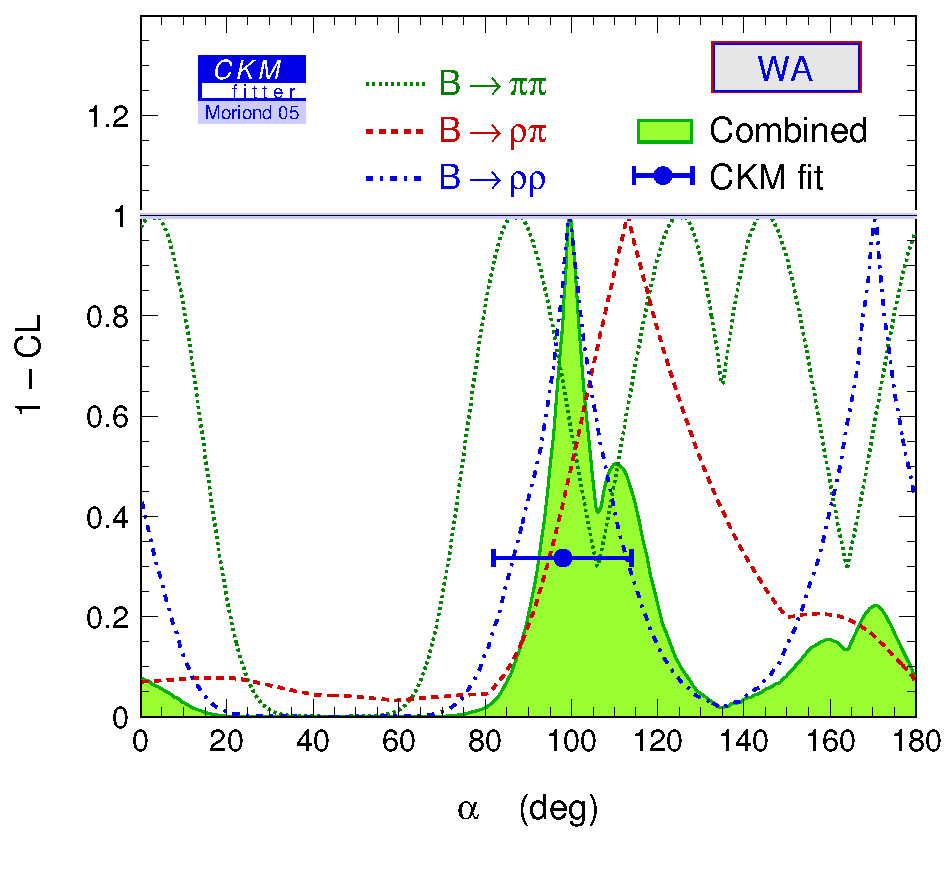
\includegraphics[width=\largefigwidth]{ckmfitter-alpha-combined}
%   \caption[CKM Fitter constraints on \alphaCKM.]%
%   {CKM Fitter constraints on \alphaCKM from combined \BToPiPi,
%     \BToRhoPi and \BToRhoRho decay analyses.}
%   \label{fig:CKMFitter}
% \end{figure}

\section{The \LHCb experiment}
\label{sec:LHCbInDetail}

Since both \bhadron{s} are preferentially produced in the same direction
and are forward-boosted along the beam-pipe, the detector is not required
to have full $4\pi$ solid-angle coverage. \LHCb takes advantage of this
by using a wedge-shaped single-arm detector with angular acceptance
\unit{10-300}{\mrad} in the horizontal (bending) plane~\cite{Amato:1998xt}.

\vspace{1cm}

\begin{center}
{\hspace{1mm}\Large\vdots\hspace{1cm}}
\end{center}

\vspace{1cm}

The detector is illustrated in \FigureRef{fig:LHCbCrossSection}, showing
the overall scale of the experiment and the surrounding cavern structure.

\begin{sidewaysfigure}
  \begin{center}
  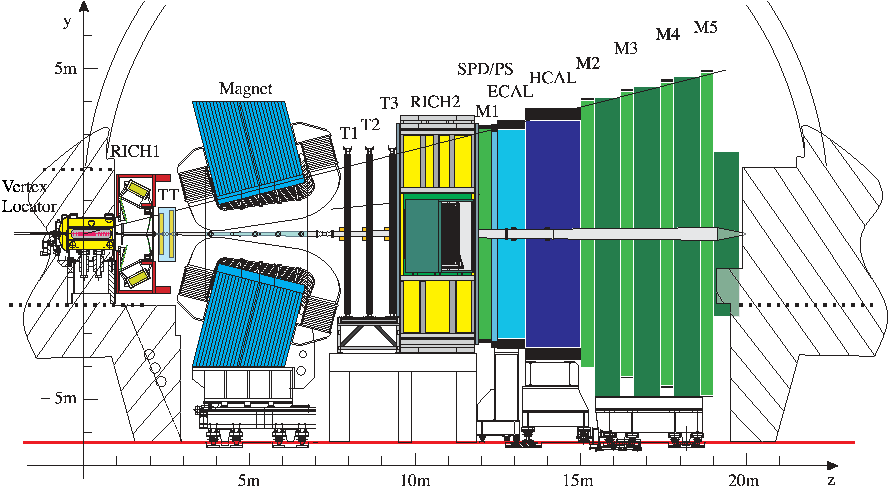
\includegraphics[width=0.8\textheight]{lhcb-detector-cross-section}
  \caption[Cross-section view of \LHCb, cut in the non-bending $y$--$z$ plane]%
    {Cross-section view of \LHCb, cut in the non-bending $y$--$z$ plane.}
  \label{fig:LHCbCrossSection}
  \end{center}
\end{sidewaysfigure}

The single-sided detector design was chosen in preference to a two-armed
design since the detector dimensions are restricted by the layout of the
IP8 (ex-Delphi) cavern in which \LHCb is located. Using all the available
space for a single-arm spectrometer more than compensates in performance
for the \about{50\percent} drop in luminosity.

\section{The \Cerenkov mechanism}
A Huygens construction in terms of spherical shells of probability for photon
emission as the particle progresses along its track shows an effective
``shock-front'' of \Cerenkov emission. This corresponds to an emission cone of
opening angle \thetaCerenkov around the momentum vector for each point on the
track,
%
\begin{subequations}
  \label{eq:cosThetaCk}
  \begin{equation}
    \cos\,\thetaCerenkov  &= \frac{1}{n \beta} +
                             \frac{\hbar k}{2p}%
                             \parenths{ 1 - \frac{1}{n^2} } \\
                          &\,\sim \frac{1}{n \beta}%
    \label{eq:cosThetaCkApprox}
  \end{equation}
\end{subequations}
%
where $\beta \equiv v/c$, the relativistic velocity fraction.

\section{Trigger system}
\label{sec:triggers}
An overview of the \LHCb trigger characteristics broken down by level
is shown in \Table~\ref{tab:TriggerDetails}.

\begin{table}[bp]
  \begin{tabular}{lllll}
                & L0              & L1              & HLT             \\
    \midrule\\
    Input rate  & \unit{40}{\MHz} & \unit{1}{\MHz}  & \unit{40}{\kHz} \\
    Output rate & \unit{1}{\MHz}  & \unit{40}{\kHz} & \unit{2}{\kHz}  \\
    Location    & On detector     & Counting room   & Counting room   \\
  \end{tabular}
  \caption{Characteristics of the trigger levels and offline analysis.}
  \label{tab:TriggerDetails}
\end{table}

  \chapter{Continued captions}
\label{chap:ContCaptions}

Here are some funky floats using ``continued captions'', i.e. for a semantically
collected group of float contents which are too numerous to fit into a single
float, such as the pretty circles in the following figure:

\newcommand{\circleimg}[1]{%
\begin{tikzpicture}
  \draw[color=black,fill=#1,thick] (1,0) circle (1.5cm);
\end{tikzpicture}%
}

\begin{figure}[hb]
  \subfloat[][Example 1a]{\label{fig:cc1a}\circleimg{red!80}}\quad
  \subfloat[][Example 1b]{\label{fig:cc1b}\circleimg{green!70!yellow}}\quad
  \subfloat[][Example 1c]{\label{fig:cc1c}\circleimg{blue!80}}\quad
  \subfloat[][Example 1d]{\label{fig:cc1d}\circleimg{orange!80!yellow}}
  \caption{Demonstration of \texttt{subfig} continued captions.}
  \label{fig:cc1}
\end{figure}

\begin{figure}[p]
  \ContinuedFloat
  \subfloat[][Example 1e]{\label{fig:cc1e}\circleimg{violet}}\quad
  \subfloat[][Example 1f]{\label{fig:cc1f}\circleimg{cyan}}\quad
  \subfloat[][Example 1g]{\label{fig:cc1g}\circleimg{magenta}}\quad
  \subfloat[][Example 1h]{\label{fig:cc1h}\circleimg{yellow}}
  \caption[]{Demonstration of \texttt{subfig} continued captions (continued).}
\end{figure}

\noindent
This mechanism means that the same float label is used for both pages of
floats. Note that we can refer to \FigureRef{fig:cc1} in general, or to
\FigureRef{fig:cc1g} on \PageRef{fig:cc1g} in particular!

\noindent
Just for the hell of it, let's also refer to \SectionRef{sec:neutralmixing}.

  %% To ignore a specific chapter while working on another, making the build faster, comment it out:
  %\input{chap4}
\end{mainmatter}

%% Produce the appendices
\begin{appendices}
  %% The "\appendix" call has already been made in the declaration
%% of the "appendices" environment (see thesis.tex).
\chapter{Pointless extras}
\label{app:Pointless}

\chapterquote{%
Le savant n'\'etudie pas la nature parce que cela est utile; \\
\indent il l'\'etudie parce qu'il y prend plaisir, \\
\indent et il y prend plaisir parce qu'elle est belle.}%
{Henri Poincar\'e, 1854--1912}

Appendixes (or should that be ``appendices''?) make you look really clever, 'cos
it's like you had more clever stuff to say than could be fitted into the main
bit of your thesis. Yeah. So everyone should have at least three of them\dots

\section{Like, duh}
\label{sec:Duh}
Padding? What do you mean?

\section{$y = \alpha x^2$}
\label{sec:EqnTitle}
See, maths in titles automatically goes bold where it should (and check the
table of contents: it \emph{isn't} bold there!) Check the source: nothing
needs to be specified to make this work. Thanks to Donald Arsenau for the
teeny hack that makes this work.

%% Big appendixes should be split off into separate files, just like chapters
%\input{app-myreallybigappendix}

\end{appendices}

%% Produce the un-numbered back matter (e.g. colophon,
%% bibliography, tables of figures etc., index...)
\begin{backmatter}
  \begin{colophon}
  This thesis was made in \LaTeXe{} using the ``hepthesis'' class~\cite{hepthesis}.
\end{colophon}

%% You're recommended to use the eprint-aware biblio styles which
%% can be obtained from e.g. www.arxiv.org. The file mythesis.bib
%% is derived from the source using the SPIRES Bibtex service.
\bibliographystyle{h-physrev}
\bibliography{mythesis}

%% I prefer to put these tables here rather than making the
%% front matter seemingly interminable. No-one cares, anyway!
\listoffigures
\listoftables

%% If you have time and interest to generate a (decent) index,
%% then you've clearly spent more time on the write-up than the 
%% research ;-)
%\printindex

\end{backmatter}

%% Close
\end{document}
